%%%%%%%%%%%%%%%%%%%%%%%%%%%%%%%%%%%%%%%%%%%%%%%%%%%%%%%%%%%%%%%%%%%%%%%%%%%%%%%%%%%%%%%%%%%%%%%%
%
% CS484 Written Question Template
%
% Acknowledgements:
% The original code is written by Prof. James Tompkin (james_tompkin@brown.edu).
% The second version is revised by Prof. Min H. Kim (minhkim@kaist.ac.kr).
%
% This is a LaTeX document. LaTeX is a markup language for producing 
% documents. Your task is to fill out this document, then to compile 
% it into a PDF document. 
%
% 
% TO COMPILE:
% > pdflatex thisfile.tex
%
% If you do not have LaTeX and need a LaTeX distribution:
% - Personal laptops (all common OS): www.latex-project.org/get/
% - We recommend latex compiler miktex (https://miktex.org/) for windows,
%   macTex (http://www.tug.org/mactex/) for macOS users.
%   And TeXstudio(http://www.texstudio.org/) for latex editor.
%   You should install both compiler and editor for editing latex.
%   The another option is Overleaf (https://www.overleaf.com/) which is 
%   an online latex editor.
%
% If you need help with LaTeX, please come to office hours. 
% Or, there is plenty of help online:
% https://en.wikibooks.org/wiki/LaTeX
%
% Good luck!
% Min and the CS484 staff
%
%%%%%%%%%%%%%%%%%%%%%%%%%%%%%%%%%%%%%%%%%%%%%%%%%%%%%%%%%%%%%%%%%%%%%%%%%%%%%%%%%%%%%%%%%%%%%%%%
%
% How to include two graphics on the same line:
% 
% \includegraphics[width=0.49\linewidth]{yourgraphic1.png}
% \includegraphics[width=0.49\linewidth]{yourgraphic2.png}
%
% How to include equations:
%
% \begin{equation}
% y = mx+c
% \end{equation}
% 
%%%%%%%%%%%%%%%%%%%%%%%%%%%%%%%%%%%%%%%%%%%%%%%%%%%%%%%%%%%%%%%%%%%%%%%%%%%%%%%%%%%%%%%%%%%%%%%%

\documentclass[11pt]{article}

\usepackage[english]{babel}
\usepackage[utf8]{inputenc}
\usepackage[colorlinks = true,
            linkcolor = blue,
            urlcolor  = blue]{hyperref}
\usepackage[a4paper,margin=1.5in]{geometry}
\usepackage{stackengine,graphicx}
\usepackage{fancyhdr}
\setlength{\headheight}{15pt}
\usepackage{microtype}
\usepackage{times}
\usepackage{booktabs}
\usepackage{graphicx}

% From https://ctan.org/pkg/matlab-prettifier
\usepackage[numbered,framed]{matlab-prettifier}

\frenchspacing
\setlength{\parindent}{0cm} % Default is 15pt.
\setlength{\parskip}{0.3cm plus1mm minus1mm}

\pagestyle{fancy}
\fancyhf{}
\lhead{Homework Writeup}
\rhead{CSCI 1430}
\rfoot{\thepage}

\date{}

\title{\vspace{-1cm}Homework X Writeup}


\begin{document}
\maketitle
\vspace{-3cm}
\thispagestyle{fancy}

\section*{Instructions}
\begin{itemize}
  \item Describe any interesting decisions you made to write your algorithm.
  \item Show and discuss the results of your algorithm.
  \item Feel free to include code snippets, images, and equations.
  \item Use as many pages as you need, but err on the short side If you feel you only need to write a short amount to meet the brief, th
  
  \item \textbf{Please make this document anonymous.}
\end{itemize}
\newcommand\tab[1][1cm]{\hspace*{#1}}
\section*{Files...}  

{\large $1.$ my\_imfilter.m \par}
\tab input : image, filter \\
\tab output : after filter image

\tab $1)$ Pad the input image with zeros. \\
\tab $2)$ Support grayscale and color images. \\
\tab $3)$ Support arbitrary shaped odd-dimension filters \\ \tab (e.g., $7x9$ filters but not $4x5$ filters). \\
\tab $4)$ Return an error message for even filters, as their output is undefined. \\
\tab $5)$ Return an identical image with an identity filter. \\
\tab $6)$ Return a filtered image which is the same resolution as the input image. \\
\tab Used in hw$2$\_test\_filtering and gen\_hybrid\_image.

{\large $2.$ hw$2$\_test\_filtering.m \par}
\tab Nothing to modify. This is to verify that my\_imfilter is fuctioning properly.

{\large $3.$ gen\_hybrid\_image.m \par}
\tab input : image$1$, image$2$, cutoff\_frequency \\
\tab output : three images [hybrid\_image,low\_frequencies,high\_frequencies] \\
\tab Just use what filters to make high pass filter and low pass filter. \\ \tab Used in vis\_hybrid\_image and hw$2$.

{\large $4.$ vis\_hybrid\_image.m \par}
\tab Nothing to modify. Adjust the scale and padding. 

{\large $5.$ hw$2$.m  \par}
\tab Nothing to modify. Using gen\_hybrid\_image and vis\_hybrid\_image, apply high pass filter and low pass filter, make hybrid image, and store each image.


\section*{In code.}
{\large $1.$ my\_imfilter.m \par}
\begin{lstlisting}[style=Matlab-editor]
function output = my_imfilter(image, filter)
\%%%%%%%%%%%%%%%%
\% Your code here

double_image = im2double(image);
[im,in,ik] = size(double_image);
[fm,fn] = size(filter);

\%if size of filter even, catch error.
if rem(fm,2)~=1
    msg = 'filter size error1.';
    error(msg);
elseif rem(fn,2)~=1
    msg = 'fliter size error2.';
    error(msg);
end

\%boundaries make zero.
cal_image = double_image;
lrzero = zeros(im,fix(fn/2),3);
cal_image = [lrzero cal_image lrzero];
udzero = zeros(fix(fm/2),in+fn-1,3);
cal_image = [udzero;cal_image;udzero];

\%calculate filter*image.
startm = fix(fm/2)+1;
endm = startm+im-1;
startn = fix(fn/2)+1;
endn = startn+in-1;
h = zeros(im,in,ik);
for i = startm:endm
    for j = startn:endn
        sum = zeros(1,ik);
        for a = 1:ik    
            temp = sum(a);
            for k = -fix(fm/2):fix(fm/2)
                for l = -fix(fn/2):fix(fn/2)
                    increase = filter(k+fix(fm/2)+1,l+fix(fn/2)+1).*cal_image(i-k,j-l,a);
                    sum(a) = temp + increase;
                    temp = sum(a);
                end
            end
            h(i-fix(fm/2),j-fix(fn/2),a) = sum(a);
        end
    end
end

output = h;
%%%%%%%%%%%%%%%%
\end{lstlisting}

Initially, if the filter was even in size, the error was detected.\\ Second, since the data can be lost when applying filter, assuming the filter size is 2m+1, 2n+1, we made each m up and down, and  each n left and right.\\ Finally, the equation for the resolution is as follows, so the process was applied to all parts of the image, not to the Boundaries.\\
convolution : \begin{Large} $$h[m,n] = \sum_{k,l} f[k,l]I[m-k,n-l]$$ \end{Large}\\\\

{\large $2.$ hw$2$\_test\_filtering.m \par}
\tab Nothing to modify. So the code will be omitted.\\\\


{\large $3.$ gen\_hybrid\_image.m \par}
\begin{lstlisting}[style=Matlab-editor]
function [hybrid_image,low_frequencies,high_frequencies] = gen_hybrid_image( image1, image2, cutoff_frequency )
\%%%%%%%%%%%%%%%%%%%%%%%
\% Remove the high frequencies from image1 by blurring it. The amount of
\% blur that works best will vary with different image pairs
\%%%%%%%%%%%%%%%%%%%%%%%
filter = fspecial('Gaussian', cutoff_frequency*4+1, cutoff_frequency);
image1 = im2double(image1);
low_frequencies = my_imfilter(image1, filter);

\%%%%%%%%%%%%%%%%%%%%%%%
\% Remove the low frequencies from image2. The easiest way to do this is to
\% subtract a blurred version of image2 from the original version of image2.
\% This will give you an image centered at zero with negative values.
\%%%%%%%%%%%%%%%%%%%%%%%
image2 = im2double(image2);
high_frequencies = image2 - my_imfilter(image2, filter);

\%%%%%%%%%%%%%%%%%%%%%%%
\% Combine the high frequencies and low frequencies
\%%%%%%%%%%%%%%%%%%%%%%%
hybrid_image = imfuse(low_frequencies,high_frequencies,'blend','Scaling','joint');
\end{lstlisting}

The low-pass filter was applied to the Gausian filter because it had to be put in blur, and the high-pass filter was made to subtract the low-pass filter from the original because only the high frequencies must remain.\\\\

{\large $4.$ vis\_hybrid\_image.m \par}
\tab Nothing to modify. So the code will be omitted.\\\\


{\large $5.$ hw$2$.m  \par}
\tab Nothing to modify. So the code will be omitted.\\\\

\pagebreak
\section*{Result...}  

{\large $1.$ my\_imfilter.m \par}
\tab Nothing output image.

{\large $2.$ hw$2$\_test\_filtering.m \par}
[output] \\
$(1)$ identity\_image.jpg
\begin{lstlisting}[style=Matlab-editor]
identity_filter = [0 0 0; 0 1 0; 0 0 0];
identity_image = my_imfilter(test_image, identity_filter);
\end{lstlisting}
\begin{figure}[!h]
    \centering
    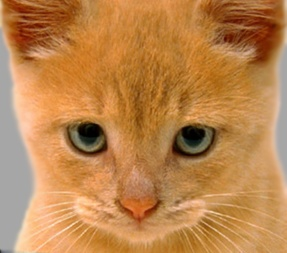
\includegraphics[width=5cm]{identity_image.jpg}
    \caption{identity\_image.}
    \label{fig:result1}
\end{figure}

$(2)$ blur\_image.jpg
\begin{lstlisting}[style=Matlab-editor]
blur_filter = [1 1 1; 1 1 1; 1 1 1];
blur_filter = blur_filter / sum(sum(blur_filter));
blur_image = my_imfilter(test_image, blur_filter);
\end{lstlisting}
\begin{figure}[!h]
    \centering
    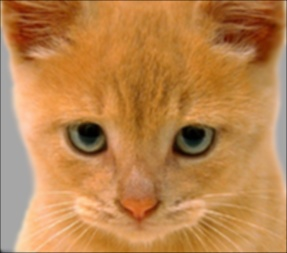
\includegraphics[width=5cm]{blur_image.jpg}
    \caption{blur\_image.}
    \label{fig:result2}
\end{figure}
\pagebreak
$(3)$ large\_blur\_image.jpg
\begin{lstlisting}[style=Matlab-editor]
large_1d_blur_filter = fspecial('Gaussian', [25 1], 10);
large_blur_image = my_imfilter(test_image, large_1d_blur_filter);
large_blur_image = my_imfilter(large_blur_image, large_1d_blur_filter');
\end{lstlisting}
\begin{figure}[!h]
    \centering
    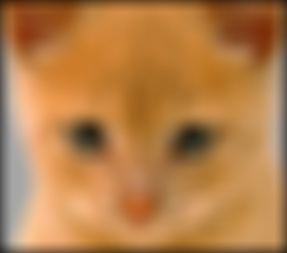
\includegraphics[width=5cm]{large_blur_image.jpg}
    \caption{large\_blur\_image.}
    \label{fig:result3}
\end{figure}

$(4)$ sobel\_image.jpg
\begin{lstlisting}[style=Matlab-editor]
sobel_filter = [-1 0 1; -2 0 2; -1 0 1]; 
sobel_image = my_imfilter(test_image, sobel_filter);
\end{lstlisting}
\begin{figure}[!h]
    \centering
    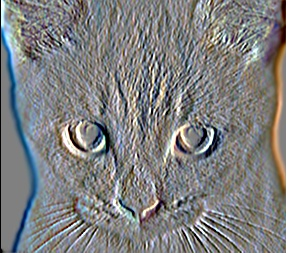
\includegraphics[width=5cm]{sobel_image.jpg}
    \caption{sobel\_image.}
    \label{fig:result4}
\end{figure}
\pagebreak
$(5)$ laplacian\_image.jpg
\begin{lstlisting}[style=Matlab-editor]
laplacian_filter = [0 1 0; 1 -4 1; 0 1 0];
laplacian_image = my_imfilter(test_image, laplacian_filter);
\end{lstlisting}
\begin{figure}[!h]
    \centering
    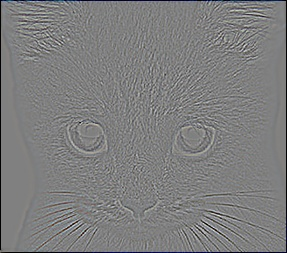
\includegraphics[width=5cm]{laplacian_image.jpg}
    \caption{sobel\_image.}
    \label{fig:result5}
\end{figure}

$(6)$ high\_pass\_image.jpg
\begin{lstlisting}[style=Matlab-editor]
high_pass_image = test_image - blur_image; 
\end{lstlisting}
\begin{figure}[!h]
    \centering
    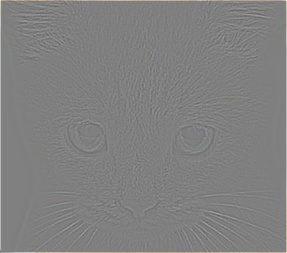
\includegraphics[width=5cm]{high_pass_image.jpg}
    \caption{high\_pass\_image.}
    \label{fig:result6}
\end{figure}
{\large $3.$ gen\_hybrid\_image \par}
\tab Nothing output image.

{\large $4.$ vis\_hybrid\_image \par}
\tab Nothing output image. 

\pagebreak
{\large $5.$ hw$2$  \par}
low\_frequencies, high\_frequencies, and hybrid\_image is made through gen\_hybrid\_image, and hybrid\_image\_scales through vis\_hybrid\_image.

[output] \\
$(1)$ low\_frequencies.jpg
\begin{lstlisting}[style=Matlab-editor]
filter = fspecial('Gaussian', cutoff_frequency*4+1, cutoff_frequency);
low_frequencies = my_imfilter(image1, filter);
\end{lstlisting}
\begin{figure}[!h]
    \centering
    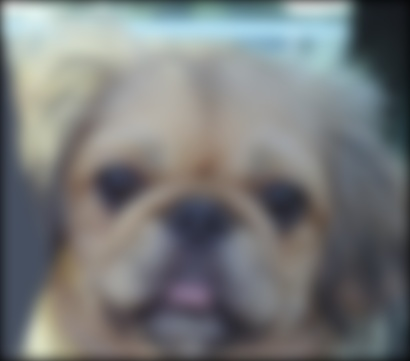
\includegraphics[width=5cm]{low_frequencies.jpg}
    \caption{low\_frequencies.}
    \label{fig:result1}
\end{figure}

$(2)$ high\_frequencies.jpg
\begin{lstlisting}[style=Matlab-editor]
high_frequencies = image2 - my_imfilter(image2, filter);
\end{lstlisting}
\begin{figure}[!h]
    \centering
    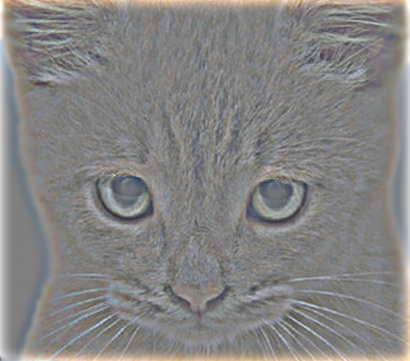
\includegraphics[width=5cm]{high_frequencies.jpg}
    \caption{high\_frequencies.}
    \label{fig:result2}
\end{figure}
\pagebreak
$(3)$ hybrid\_image.jpg
\begin{lstlisting}[style=Matlab-editor]
hybrid_image = imfuse(low_frequencies,high_frequencies,'blend','Scaling','joint');
\end{lstlisting}
\begin{figure}[!h]
    \centering
    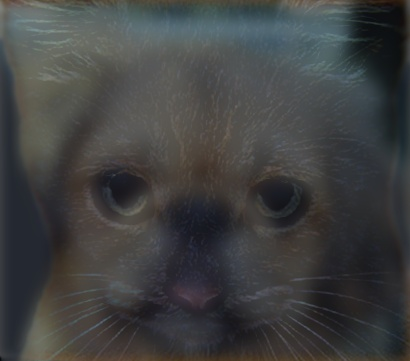
\includegraphics[width=5cm]{hybrid_image.jpg}
    \caption{hybrid\_image.}
    \label{fig:result3}
\end{figure}

$(4)$ hybrid\_image\_scales.jpg
\begin{lstlisting}[style=Matlab-editor]
scales = 5; 
scale_factor = 0.5; 
padding = 5; 

original_height = size(hybrid_image,1);
num_colors = size(hybrid_image,3); 
output = hybrid_image;
cur_image = hybrid_image;

for i = 2:scales
    output = cat(2, output, ones(original_height, padding, num_colors));
    cur_image = imresize(cur_image, scale_factor, 'bilinear');
    tmp = cat(1,ones(original_height - size(cur_image,1), size(cur_image,2), num_colors), cur_image);
    output = cat(2, output, tmp);    
end
\end{lstlisting}
\begin{figure}[!h]
    \centering
    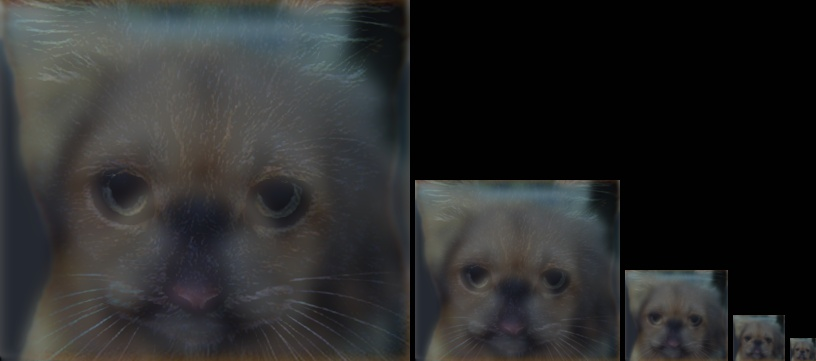
\includegraphics[width=6.5cm]{hybrid_image_scales.jpg}
    \caption{hybrid\_image\_scales.}
    \label{fig:result4}
\end{figure}

\end{document}